% (4 Seiten)
\section{Feature Evaluation}
\label{sec:FeatureEval}
This section evaluates the first and higher order features, which were described in Section \ref{sec:NEL}. The quality measures used are again precision, recall and $F_1$-Score, which were defined in Definition \ref{def_prf} and used in Section \ref{sec:ModelEval}. First, the first order features are evaluated, then the addition of all higher order features and finally every single higher order feature of the context score is evaluated. Of these evaluations, the first and last ones are done with the leave-one-out strategy to avoid a time-consuming exhaustive grid search. In the case of the first order features, there is also no other way to evaluate the link score since it is equal for all feature entries generated from the same link or trie alias. The tests were done with a Random Forest classifier, which was trained as described in Section \ref{sec:ModelEval}. It was trained with the same parameters that were used in Section \ref{sec:ModelEval}: a maximum tree depth of 6, a maximum number of bins of 40 and with 20 trees.\par

\subsection{First Order Features}
The first order features are, as described in Section \ref{sec:NEL}, the link score, entity score and context score. Figure \ref{fo_eval} shows a leave-one-out evaluation of these features. Each group of bars, which show precision, recall and $F_1$-Score, shows the quality of a model trained using the specified first order features. The model trained with all first order features is used to evaluate the other three models by comparing them to it. The other three models were trained using only two of the first order features.\par
\begin{figure}[H]
	\centering
	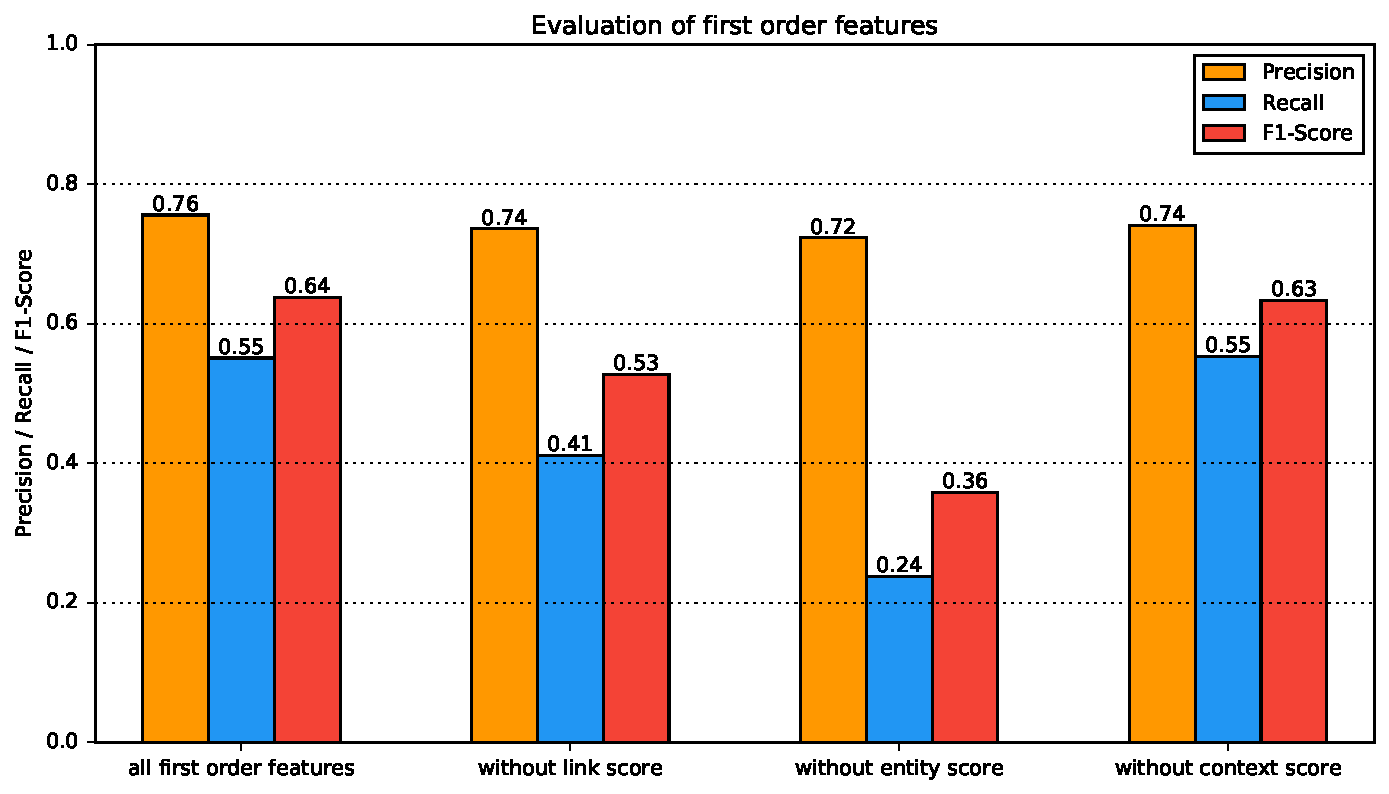
\includegraphics[width=0.9\textwidth]{img/first_order_eval}
	\caption{Leave-one-out evaluation of the first order features.}
	\label{fo_eval}
\end{figure}
The model without the link score has only $2\%$ less precision and $14\%$ less recall compared to the model with all first order features. This shows that, as intended, the link score mainly signifies whether or not the alias of a specific feature is an important word. The drop in the precision is so small because the link score can't be used to disambiguate between multiple entities one alias could link to since it is the same for all feature entries generated for one link or trie alias.\par
%In the case that all feature entries generated for an alias have small entity scores and a small cosine similarities, which are as described by Janetzki \ref{janetzki} generally small, a missing link score can lead to all feature entries being classified as negatives.
The removal of the entity score causes, compared to the model with all features, a small precision drop as well. The recall drop is a lot larger with $31\%$. Because the recall is only at $24\%$ it is not surprising that the precision drop is only relatively small. The small recall signifies that only the obvious feature entries were classified as positives. An example for such an obvious feature entry would be the alias \itcite{Commerzbank AG}. This alias occurs 125 times, of which 93 are as link, and every time it is linked it links to the page \itcite{Commerzbank}. Therefore, only one feature entry is generated for the alias and it has a high link score of $0.744$, meaning that its likely to be classified as positive. The large drop of the recall shows that the entity score is the most important feature, doing most of the disambiguation and thus entity linking. Since all the feature entries for the same alias have the same link score, only the context score would disambiguate the entities. But, as Janetzki showed, the range of the context score is relatively small, while the range of entity score is very large\ \cite{janetzki}. The small range of the context score results in a difficult disambiguation between multiple feature entries if it is the only feature used to do so.\par
The last model has very similar statistics compared to the model with all features. The small precision drop shows that the context score is used to disambiguate between feature entries of an alias with multiple very likely entities. An example would be the alias \itcite{BVB}. Out of the 340 times, it is linked in the Wikipedia, it links 107 times to the \itcite{Basler Verkehrs-Betriebe} and 208 times to \itcite{Borussia Dortmund}. This means that the entity scores are relatively similar while the context scores will most likely differ due to the entities appearing in very different contexts. E.g., \itcite{Basler Verkehrs-Betriebe} is most likely meant if the context of the alias is about traffic and \itcite{Borussia Dortmund} is most likely meant if the context is about soccer.\par
% This evaluation shows that all of the first order features improve the classification result and do that in the intended way.

\subsection{Higher Order Features}
The higher order features, which were described in Section \ref{sec:NEL}, are the rank, $\Delta top$ and $\Delta succ$. They are added to the entity score and the context score since they show the relationship between the feature entries generated from a single link or trie alias. Figure \ref{ho_eval_gen} shows the quality of four classification models. The first model was trained using only the first order features. The next two were trained with the higher order features for only a single feature. The last model was trained with the higher order features for both the entity and the context score.\par
\begin{figure}[H]
	\centering
	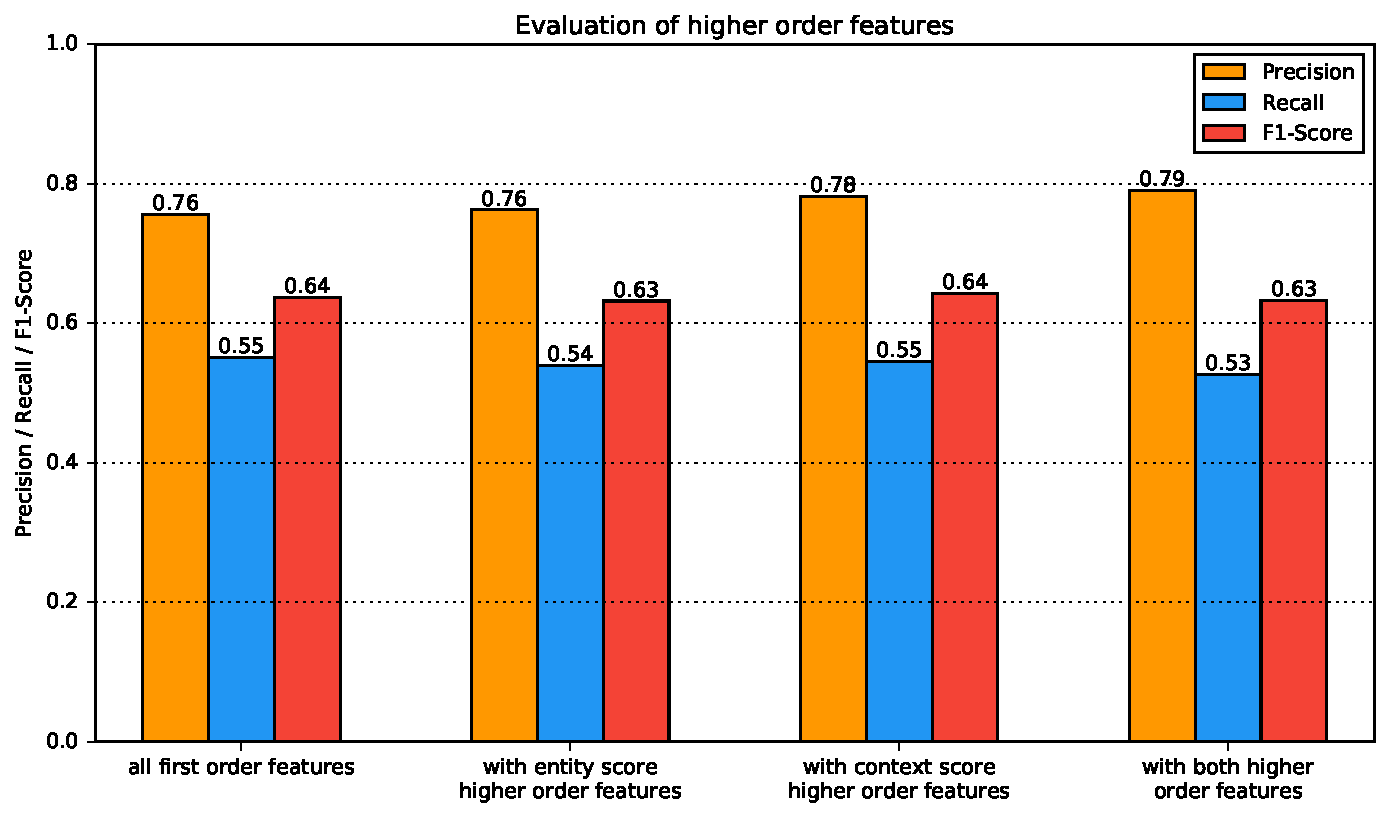
\includegraphics[width=0.9\textwidth]{img/higher_order_eval}
	\caption{Evaluation of the higher order features.}
	\label{ho_eval_gen}
\end{figure}
Adding the higher order features to the entity score did not improve the model by a lot. The precision improved by only $0.7\%$, which is not visible in Figure \ref{ho_eval_gen} due to rounding, and the recall dropped by a per cent. This demonstrates that since the entity score itself already has a very large impact on the model, the higher order features did not do so and made the model only a little more cautious. The relationship between the entity scores of multiple feature entries is in most cases already shown by the scores themselves because for many aliases there are only a few entities with a high entity score. This explains the small impact of the higher order features.\par
Adding the higher order features to the context score improves the precision by $2\%$ while dropping the recall only by $0.5\%$. The drop of the recall is again not visible due to rounding. This displays that adding the higher order features to the context score further improves the disambiguation with minimal impact on the recall. The higher order features have a higher impact on the context score compared to the entity score because, as previously said, the value range for the context score is relatively small. This causes the higher order features to bring the small values into perspective, i.e., the rank tells the classifier that a value is the best value even though it is small. The disambiguation is improved as feature entries with otherwise high scores might have the worst similarity of the words appearing around the alias and the page of the linked entity. The resulting context score is small, has a bad rank and a large $\Delta top$. Previously the difference of the context score might not have been large enough to matter but now the rank easily shows that the feature entry is a bad candidate.\par
The last model used the higher order features for both the entity and the context score. The improvement of the precision compared to the model with the higher order features for the context score shows that the higher order features for the entity score indeed improved the precision by a small amount. Likewise, the drop of the recall compared to the model with the higher order features for the entity score shows that the higher order features for the context score dropped the recall by a small amount. Overall the precision is increased by $3\%$ compared to the model without higher order features. The recall dropped by only $2\%$. This shows that while the higher order features did help improve the classifier they did so only by a small amount unlike the improvement seen by Grütze et al.\ \cite{coheel}.\par
% \subsection{Context Score's Higher Order Features}
The impact of each higher order feature on the entity score is not shown since it is minimal, which is demonstrated by the generally small impact of the entity score's higher order features. The context score's higher order features are evaluated using a leave-one-out evaluation. Figure \ref{ho_eval_context} shows the quality of four models. The first one was trained with all first and higher order features and will be used for comparison. The next three models show a model without the described higher order feature.\par
\begin{figure}[H]
	\centering
	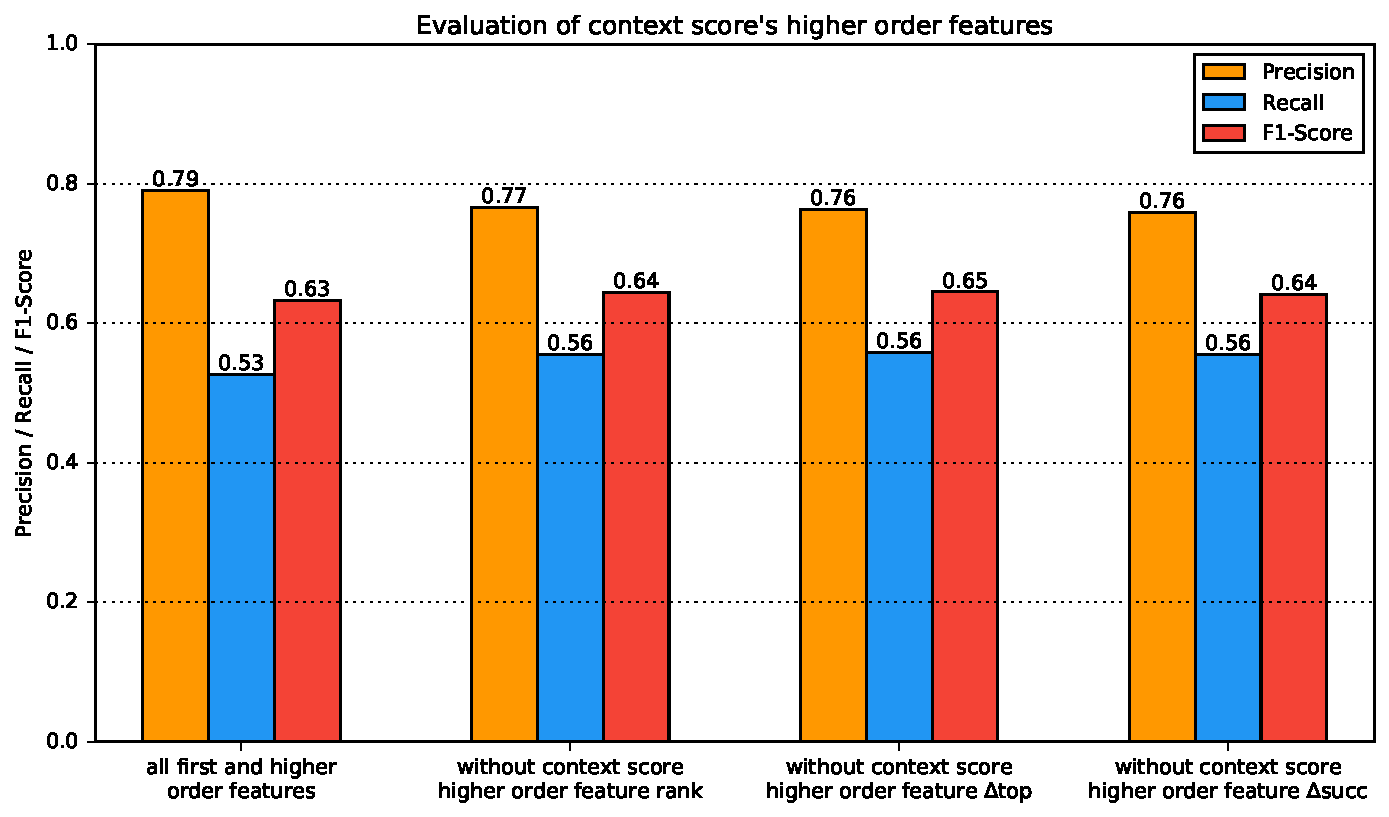
\includegraphics[width=0.9\textwidth]{img/higher_order_eval_context}
	\caption{Leave-one-out evaluation of the context score's higher order features.}
	\label{ho_eval_context}
\end{figure}
The removal of any higher order feature drops the precision by $2-3\%$ and increases the recall by $3\%$. While not visible, the largest impact has $\Delta succ$. Its removal drops the precision by $0.3\%$ more than the removal of $\Delta top$. This evaluation demonstrates that the higher order features work best when using all of them together, an observation Grütze et al. made as well\ \cite{coheel}.

% \begin{figure}[H]
% 	\centering
% 	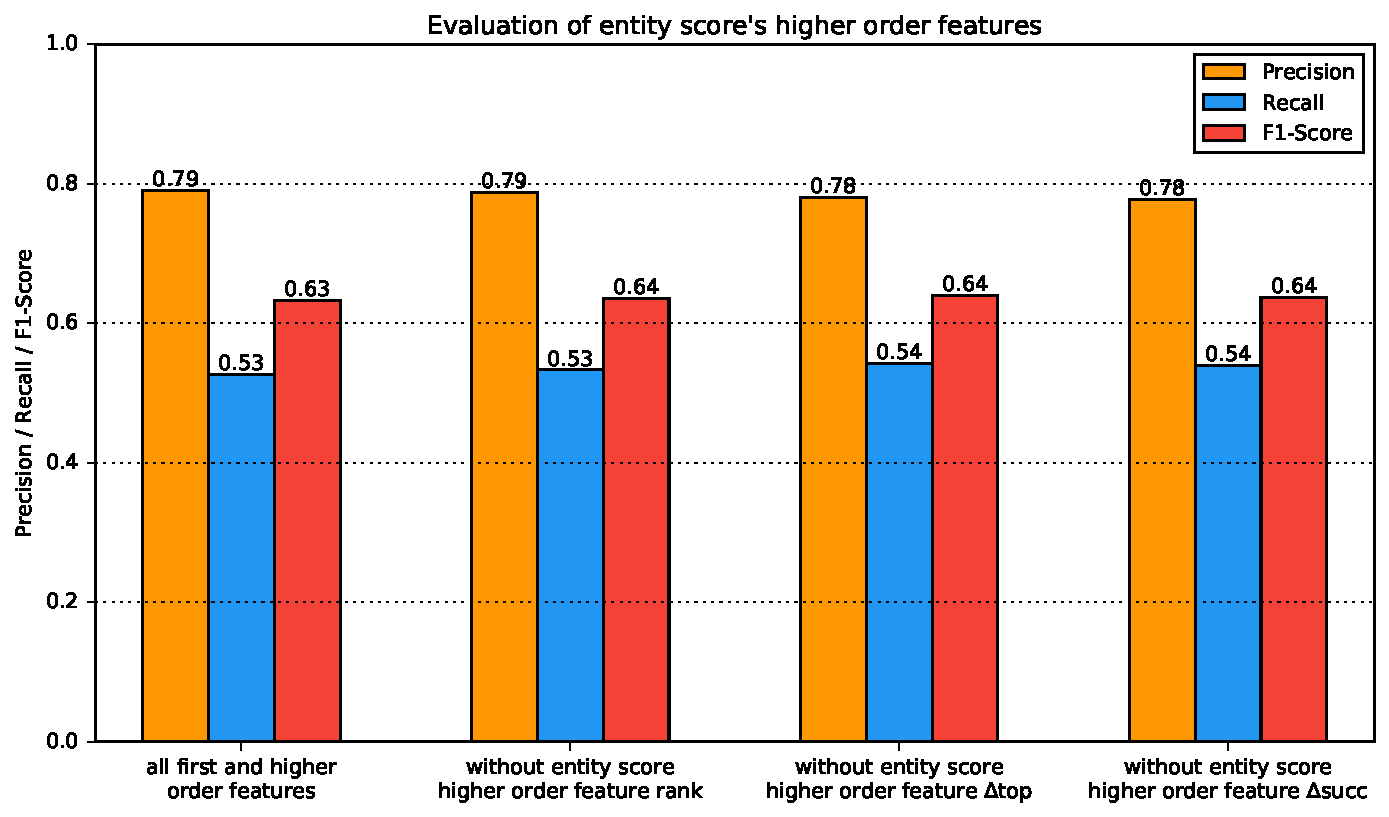
\includegraphics[width=0.9\textwidth]{img/higher_order_eval_entity}
% 	\caption{Leave-one-out evaluation of the entity score's higher order features.}
% 	\label{ho_eval_entity}
% \end{figure}